\documentclass[11pt]{article}
%ACENTOS
\usepackage[utf8]{inputenc}
\def\figurename{Fig.}
\def\tablename{Tabla}
\def\refname{Referencias}
\setlength{\parskip}{1em}

%PAQUETES
\usepackage{amsfonts,amsmath,amssymb}    % need for subequations
\usepackage{amsmath,latexsym}
\usepackage{graphics,color}
\usepackage{graphicx}
\usepackage{algpseudocode}
\usepackage[most]{tcolorbox}
\usepackage{hyperref} %Para colocar direcciones Web
\usepackage{booktabs} % Tablas
\usepackage[thinc]{esdiff} % Derivadas

%MARGEN
\setlength\topmargin{-0.5in}
\addtolength\oddsidemargin{-0.5in}
\setlength{\textheight}{23cm}
\setlength{\textwidth}{16cm}

%VARIABLES
\newcommand{\N}{\mathbb N}
\newcommand{\Z}{\mathbb Z}
\newcommand{\R}{\mathbb R}
\newcommand{\C}{\mathbb C}
\providecommand{\norm}[1]{\lVert#1\rVert}
%COLORES
\newcommand{\rojo}[1]{\textcolor[rgb]{1.00,0.00,0.00}{#1}}
\newcommand{\azul}[1]{\textcolor[rgb]{0.00,0.00,1.00}{#1}}
\usepackage{empheq}

\documentclass[fleqn]{article}
\usepackage{amsmath}
  
\begin{document}

\begin{center}
 \Large \underline {\\ \\Tarea 3: Ceros de polinomios} \\ \medskip
 \small  {Elaborado por Giselt Parra}\\ 
 \footnotesize{Lunes, 2 de Noviembre de 2020.}
\end{center}


\vspace{0.75cm}
\begin{center} \large  {Propuesta: Método de Müller usando Interpolación \\Polinómica de Lagrange Simplificado} \end{center}

\vspace{0.5cm}
Para la implementación de esta propuesta se propone combinar las ventajas de la técnica de deflación de Horner tanto para evaluar puntos en los polinomios así como para generar polinomios de menor grado cuando se evalúa con una raíz así como también se implementa el método de Müller que aproxima raices de una manera similar al método de la Secante con la diferencia de que se trazan parábolas en tres puntos del polinomio. Siendo éstas representadas por ecuaciones cuadráticas, el método nos permite hallar raíces imaginarias aún cuando los iteradores iniciales son reales.


El método de Müller es un algoritmo que consiste en interpolar el polinomio $p$ en tres puntos resultando así una ecuación cuadrática que representa la parábola que pasa por estos tres puntos y que aproximará a una raíz del polinomio $p$ cuando corta con el eje x en la raíz de la parábola más cercano al tercer y último iterador calculado. Este punto de corte es un posible cero del polinomio que estamos evaluando, por lo que se hacen las comparaciones pertinentes respecto a su altura y diferencia con el iterador anterior para verificar si es una buena aproximación. De serlo, se considerará este punto una raíz y se procede a realizar una deflación tomando como valor a evaluar dicho punto que dará como resultado un nuevo polinomio de grado menor y así continuar la búsqueda de las siguientes raíces. En el caso contrario, este punto se tomará como nuevo iterador y se continuará operando de la misma forma descrita hasta hallar una buena aproximación.

\begin{center}
    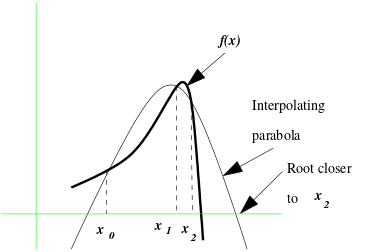
\includegraphics[keepaspectratio, width=11cm]{muller.png}
    \caption \tiny{\\ Construcción de la parábola en el método de Müller ilustrado}
\end{center}  
\vspace{0.75cm}

Para hallar el polinomio interpolante de segundo grado que usaremos en cada iteración para el método de Müller, usaremos la base Lagrange que consiste en construir una base 

$$ B_L = \{l_0(x),l_1(x),l_2(x)\}$$

donde cada $l_i$ se construye como

$$l_0(x) = \prod_{j=0,j\neq0}^{2} \frac{x-x_j}{x_0 - x_j} =
	    \frac{(x-x_1)(x-x_2)}{(x_0 - x_1)(x_0 - x_2)} 
$$
$$l_1(x)  = \prod_{j=0,j\neq1}^{2} \frac{x-x_j}{x_1 - x_j} = 
	    \frac{(x-x_0)(x-x_2)}{(x_1 - x_0)(x_1 - x_2)} 
$$
$$l_2(x)  = \prod_{j=0,j\neq2}^{2} \frac{x-x_j}{x_2 - x_j} =
	    \frac{(x-x_0)(x-x_1)}{(x_2 - x_0)(x_2 - x_1)}
$$

Ya obtenido los elementos que conforman la base, se escribe el polinomio a generar como la siguiente combinación lineal

$$p_n(x) = b_0l_0(x) + b_1l_1(x) + b_2l_2(x)$$

Cómo se puede ver, la base de Lagrange cumple que 
$$
l_i(x_j)=\begin{cases}
    1, & \mbox{si $i=j$,}\\
    0, & \mbox{si $i\neq j$.}
\end{cases}
$$

Por lo tanto, el sistema de ecuaciones que se obtiene al imponer las condiciones de interpolación $p(x_i) = y_i$ es un sistema trivial


\begin{equation*}
\begin{pmatrix}
1 & 0 & 0 \\ 
0 & 1 & 0 \\
0 & 0 & 1 \\
\end{pmatrix}
\begin{pmatrix}
b_0 \\ 
b_1 \\
b_2 \\
\end{pmatrix}
=
\begin{pmatrix}
y_0 \\ 
y_1 \\
y_2 \\
\end{pmatrix}
\end{equation*}
%?????????????????????????????????????????????????????????????????

%DE ESTA FORMA SE EVITA EL MAL CONDICIONAMIENTO ??????????????????

%?????????????????????????????????????????????????????????????????

Esto quiere decir que la solución del sistema es $b_i = y_i$ por lo que el polinomio interpolante es $p_2(x) = y_0l_0(x) + y_1l_1(x) + y_2l_2(x)$ e implica una mejora al condicionamiento del sistema.

Considerando que el objetivo del método de Müller es hallar las raíces de la función a través de aproximaciones con parábolas a la función, el polinomio interpolante será de un polinomio de segundo grado en todas las iteraciones. Sabiendo esto, se puede tomar la ventaja de utilizar la fórmula $x = \frac{-b \pm \sqrt{b^2 - 4ac}}{2a}$ para hallar raíces de ecuaciones cuadráticas y conociendo de qué manera funciona la interpolación usando bases de Lagrange, se pueden realizar manipulaciones algebraicas para calcular el valor de los coeficientes de una manera más directa.

Al calcular los elementos que conforman la base de Lagrange, se puede notar que el denominador de la productoria resultará en una constante a la que llamaremos $d_i$
$$l_0(x) = \prod_{j=0,j\neq0}^{2} \frac{x-x_j}{x_0 - x_j} =
	    \frac{(x-x_1)(x-x_2)}{(x_0 - x_1)(x_0 - x_2)} =
	     \frac{(x-x_1)(x-x_2)}{d_0}
$$
$$l_1(x)  = \prod_{j=0,j\neq1}^{2} \frac{x-x_j}{x_1 - x_j} = 
	     \frac{(x-x_0)(x-x_2)}{d_1}
$$
$$l_2(x)  = \prod_{j=0,j\neq2}^{2} \frac{x-x_j}{x_2 - x_j} =
	     \frac{(x-x_0)(x-x_1)}{d_2}
$$

Reescribimos $p_2(x) = y_0l_0(x) + y_1l_1(x) + y_2l_2(x)$ reemplazando $l_i$

$$p_2(x) = y_0\frac{(x-x_1)(x-x_2)}{d_0} + y_1\frac{(x-x_0)(x-x_2)}{d_1} + y_2\frac{(x-x_0)(x-x_1)}{d_2}
$$
expandiendo el producto de diferencias en cada numerador y tomando $m_i = \frac{y_i}{d_i}$
$$
p_2(x) =  m_0(x^2 - x(x_1+x_2) + x_1x_2) + m_1(x^2 - x(x_0+x_2) + x_0x_2) + m_2(x^2 - x(x_0+x_1) + x_0x_1)$$

de esta forma se pueden extraer los coeficientes que corresponden a cada término del polinomio de segundo grado de la forma $ax^2 + bx + c$

Al desarrollar las cuentas tenemos que:

$$a = m_0 + m_1 + m_2$$
$$b = -m_0(x_1+x_2) - m_1(x_0+x_2) - m_2(x_0+x_1)$$ 
$$c =  m_0x_1x_2 + m_1x_0x_2 + m_2x_0x_1$$ 

\vspace{0.5cm}
\begin{center} \large  {Implementación y Resultados} \end{center}

\vspace{0.25cm}
\begin{tcolorbox}[colframe=blue!35!black, title=Código]
    CerosDePolinomios.m
\end{tcolorbox}
\vspace{0.5cm}

Para la implementación en el método de Müller con el propósito de reducir la complejidad espacial, cada polinomio generado luego de realizar una depuración, se almacenará en él mismo evitando crear un nuevo arreglo de coeficientes por cada depuración. Otro aspecto considerado con el fin de hacer el algoritmo más eficiente es que la simplificación al método de Lagrange para hallar el polinomio interpolante implica realizar todos los cálculos requeridos para hallar los coeficientes del polinomio de segundo grado de manera estática, por lo que se evita el uso de ciclos para realizar las productorias correspondientes al método así como también el hecho de trabajar luego con un sistema de ecuaciones trivial que mejora el condicionamiento del sistema.

A continuación, los resultados dados por el programa junto a la gráfica de los polinomios escogidos para la prueba del método.
\begin{center}
    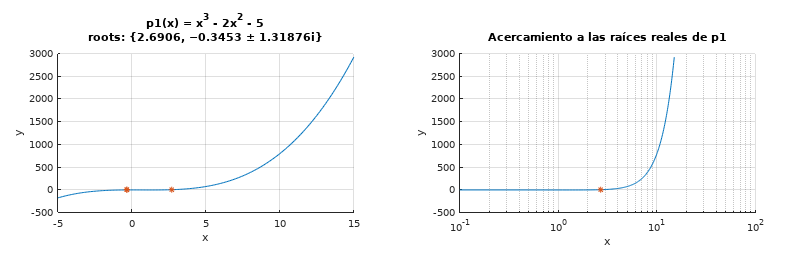
\includegraphics[keepaspectratio, width=14cm]{P1.png}
    \caption \tiny{\\Prueba al polinomio $p1_3(x) = x^3 - 2x^2 - 5$ con iteradores iniciales $x_0 = -1, x_1 = 0, x_2 = 1$
    \\Raíces obtenidas por el programa: $\{2.69065, -0.34532 - 1.31873i, -0.34532 + 1.31873i\}$
    }
    \vspace{0.5cm}
    
    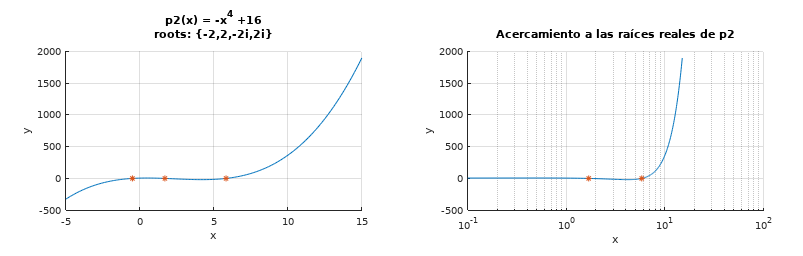
\includegraphics[keepaspectratio, width=14cm]{P2.png}
     \caption \tiny{\\Prueba al polinomio $p2_4(x) = -x^4 +16$ con iteradores iniciales $x_0 = 0, x_1 = 1, x_2 = 2$
     \\Raíces obtenidas por el programa: $\{2.00000 + 0.00000i,  -0.00000 - 2.00000i,  -0.00000 + 2.00000i,   2\}$}
     \vspace{0.5cm}
     
    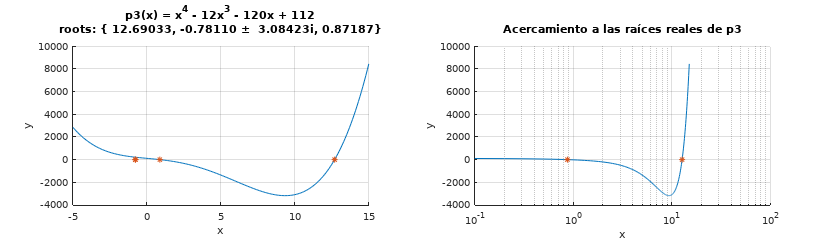
\includegraphics[keepaspectratio, width=14cm]{P3.png}
     \caption \tiny{\\Prueba al polinomio $p3_4(x) = x^4 - 12x^3 - 120x + 112$ con iteradores iniciales $x_0 = 0, x_1 = 1, x_2 = 2$
     \\Raíces obtenidas por el programa: $\{12.69033,  -0.78110 -  3.08423i,   -0.78110 +  3.08423i,    0.87187\}$}
\end{center} 

Para todas la pruebas realizadas se escogieron polinomios con raíces reales e imaginarias iniciando el algoritmo con iteradores reales para así mostrar la efectividad del método para hallar todas las raíces del polinomio sin la limitación que presentan otros métodos de escoger iteradores reales con el fin de hallar raíces reales.

\vspace{0.75cm}

\begin{center} \large  {Propuesta Adicional: Interpolación Inversa} \end{center}

Esta propuesta es similar a la expuesta previamente con la diferencia de que se construirá un polinomio $q_n$ que interpole a la inversa de la función $f$. Para esto se tomarán como nodos las alturas de los puntos dado de la función $f$.

Se plantea este camino como una solución para aproximar raíces ya que el polinomio $q_n$ evaluado en una altura de la función resulta en un punto en el dominio de f, por tanto, sólo bastará con evaluar el polinomio cuando $y = 0$ dando como resultado una aproximación a una raíz de la función. Esto simplifica mucho más el cálculo para la obtención de la raíz ya que al evaluar $q_n(y) = ay^2 + by + c$ cuando $y=0$, los primeros dos términos se multiplican por cero quedando así c como la raíz aproximada.

%?????????????????????????????????????????????????????????????????

%SINONIMO DE IMPOSIBILIDAD

%?????????????????????????????????????????????????????????????????
La razón por la que se expone esto como una alternativa y no como propuesta principal es por el incoveniente que se presenta para hallar raíces imaginarias con iteradores iniciales reales. Para explicar la razón procederemos a dar una noción visual de cómo se puede interpretar gráficamente la existencia de las raíces imaginarias en el plano cartesiano.

Se sabe que el discriminante $\Deltax = b^2 - 4ac$ de una ecuación cuadrática nos indica el número de raíces que posee. Si $\Deltax < 0$ quiere decir que la parábola que representa dicha ecuación no cortará en ningún punto del dominio con el eje x, por esta razón y sumado el hecho de que en este método se prescinde de usar la fórmula $x = \frac{-b \pm \sqrt{b^2 - 4ac}}{2a}$ para hallar raíces, sino que directamente tomamos el valor del término que representa c, no basta con que determinemos donde la función $f$ corta con el eje x.
 
Importante: Para la interpolación inversa se debe cumplir que todas las alturas $y_i$ dadas deben ser diferentes y garantizar que 
$$ f^{-1}(y_i) = x_i$$
Si ocurre que dado un $y_s$, si $f^{-1}(y_s)$ posee dos valores diferentes, entonces $f^{-1}$ no es una función.




\vspace{1cm}	
%bibliografia
\begin{thebibliography}{9}

\bibitem{se} 
Ward Cheney y David Kincaid.
\textit{Numerical Mathematics and Computing, Sixth edition}. 
The University of Texas at Austin.

\bibitem{fi} 
Michael T. Heath. 
\textit{Scientific Computing: An Introductory Survey.}. 
University of Illinois at Urbana-Champaign, 1997.

\bibitem{se} 
Biswa N. Datta, Luis M. Hernández-Ramos y Marcos Raydan.
\textit{Análisis Numérico. Teoría y Práctica}. 
[2018]

\end{thebibliography}

\end{document}